Mehr zu den ``Clean Architecture'' kann man im Buch ... lesen.

Die Architecture besteht aus konzentrischen Kreisen. Die Kreise repräsentieren verschiede Aufgaben, die eine Anwendung erledigen kann.
In der Abbildung \ref{fig:Clean Architecture} sind vier Kreise dargestellt. Die Anzahl an Kreisen kann sich variieren, solange Dependency Rule erfüllt wird.

Dependency Rule besagt, dass die Kreise keine äußeren Kreise benutzen dürfen.

Folgende Eigenschaften hat diese Architektur laut Robert Martin:
\begin{itemize}
    \item Unabhängig von dem Framework
    \item Testbar
    \item Unabhängig von der UI
    \item Unabhängig von der Datenbank
    \item Unabhängig von jeder externen Schnittstelle
\end{itemize}

\begin{figure}[H]
    \centering
    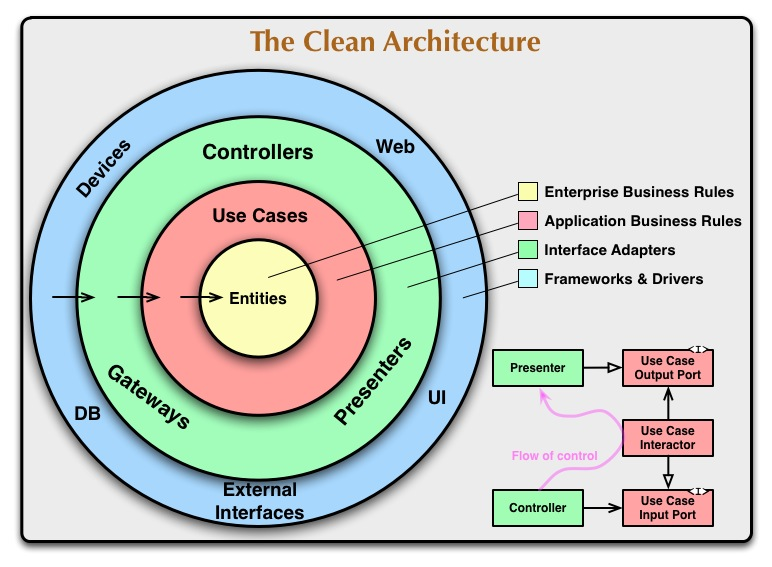
\includegraphics[width=1\textwidth]{./images/CleanArchitecture.jpg}
    \caption[Clean Architecture]{Clean Architecture \footnotemark}
    \label{fig:Clean Architecture}
\end{figure}
\footnotetext{https://blog.cleancoder.com/uncle-bob/2012/08/13/the-clean-architecture.html}